% Allow relative paths in included subfiles that are compiled separately
% See https://tex.stackexchange.com/questions/153312/

\providecommand{\main}{..}
\documentclass[\main/thesis.tex]{subfiles}
\externaldocument{}


\begin{document}
\chapter{Making Noise, Hearing Drums}
\label{implementation}


\section{Our Goal}
Our goal is to create a system for the generation of novel drum sounds. In this chapter, we will discuss the two main components of our system: The \textit{virtual synthesizer} and the \textit{virtual ear}. A quick outline of our generative pipeline is this: The virtual synthesizer will rapidly generate random programs and the corresponding sounds. As the virtual synthesizer creates sounds based on these programs, the virtual ear will listen to the sounds and determine if they should be categorized as drums and if so, which category of drum do they belong to. In case of search, other algorithms can create programs for the synthesizer and receive the rating/categorization assigned by the virtual ear. A visual representation of our pipeline is illustrated in  figure~\ref{fig:pipeline_outline}.

In Section~\ref{vs} we discuss the implementation of a virtual synthesizer which can create a wide variety of noise. We believe that a number of these noise samples can be substituted for drums of various categories. We refer to the set of synthetic noise samples which can be considered novel drums as $\mathcal{N}$. The task of the virtual ear is to listen to the outputs of the virtual synthesizer and extract the samples belonging to $\mathcal{N}$ with the highest possible precision and recall. When our pipeline is constructed, we expose the ear to a number of synthetic noises and observe the extracted sounds. We call this procedure a hearing test, and the set of sounds received by the ear $\mathcal{H}$. 

To train an effective synthetic ear, there are a variety of sound groups which need to be accounted for. For examples, a common feature shared in percussive sounds is the quick \emph{attack} (rise in volume) at the onset of impact followed by an instant, continuous \emph{decay} (drop in volume) until silence is reached~\cite{barry2005drum}. For a virtual ear to learn these and other common features, we require a set of examples for what drums do and do not sound like. The synthetic ear needs to separate drum sounds from \enquote{not-drum} sounds and categorize various types of drums. We call these tasks \enquote{DVN} and \enquote{DVD} respectively. We train our models by example, therefore, any given set of training data $\mathcal{T}$ must have an adequate number of positive ($\mathcal{T^{+}}$) and negative ($\mathcal{T^{-}}$) examples. We can use manually labeled data-sets of drums to extract features unique to percussive sounds. Can we non-tautologically describe what features are unique and common in non-percussive sounds? In this work, we seek to represent not-drums using a relatively small subset of sounds output by the virtual synthesizer. We consider the search for the succinct representation of $\mathcal{T^{-}}$ as a significant hurdle in our implementation.


\\
In this chapter we discuss in more detail the implementations and interactions of these two components. Details about the data-sets and code which can be used for replication of each part of the project can be found in Section~\ref{sec:data}.

 \begin{figure}[t!]
    \begin{center}
    \textbf{Pipeline Design}
    \makebox[\textwidth]{
    \fbox{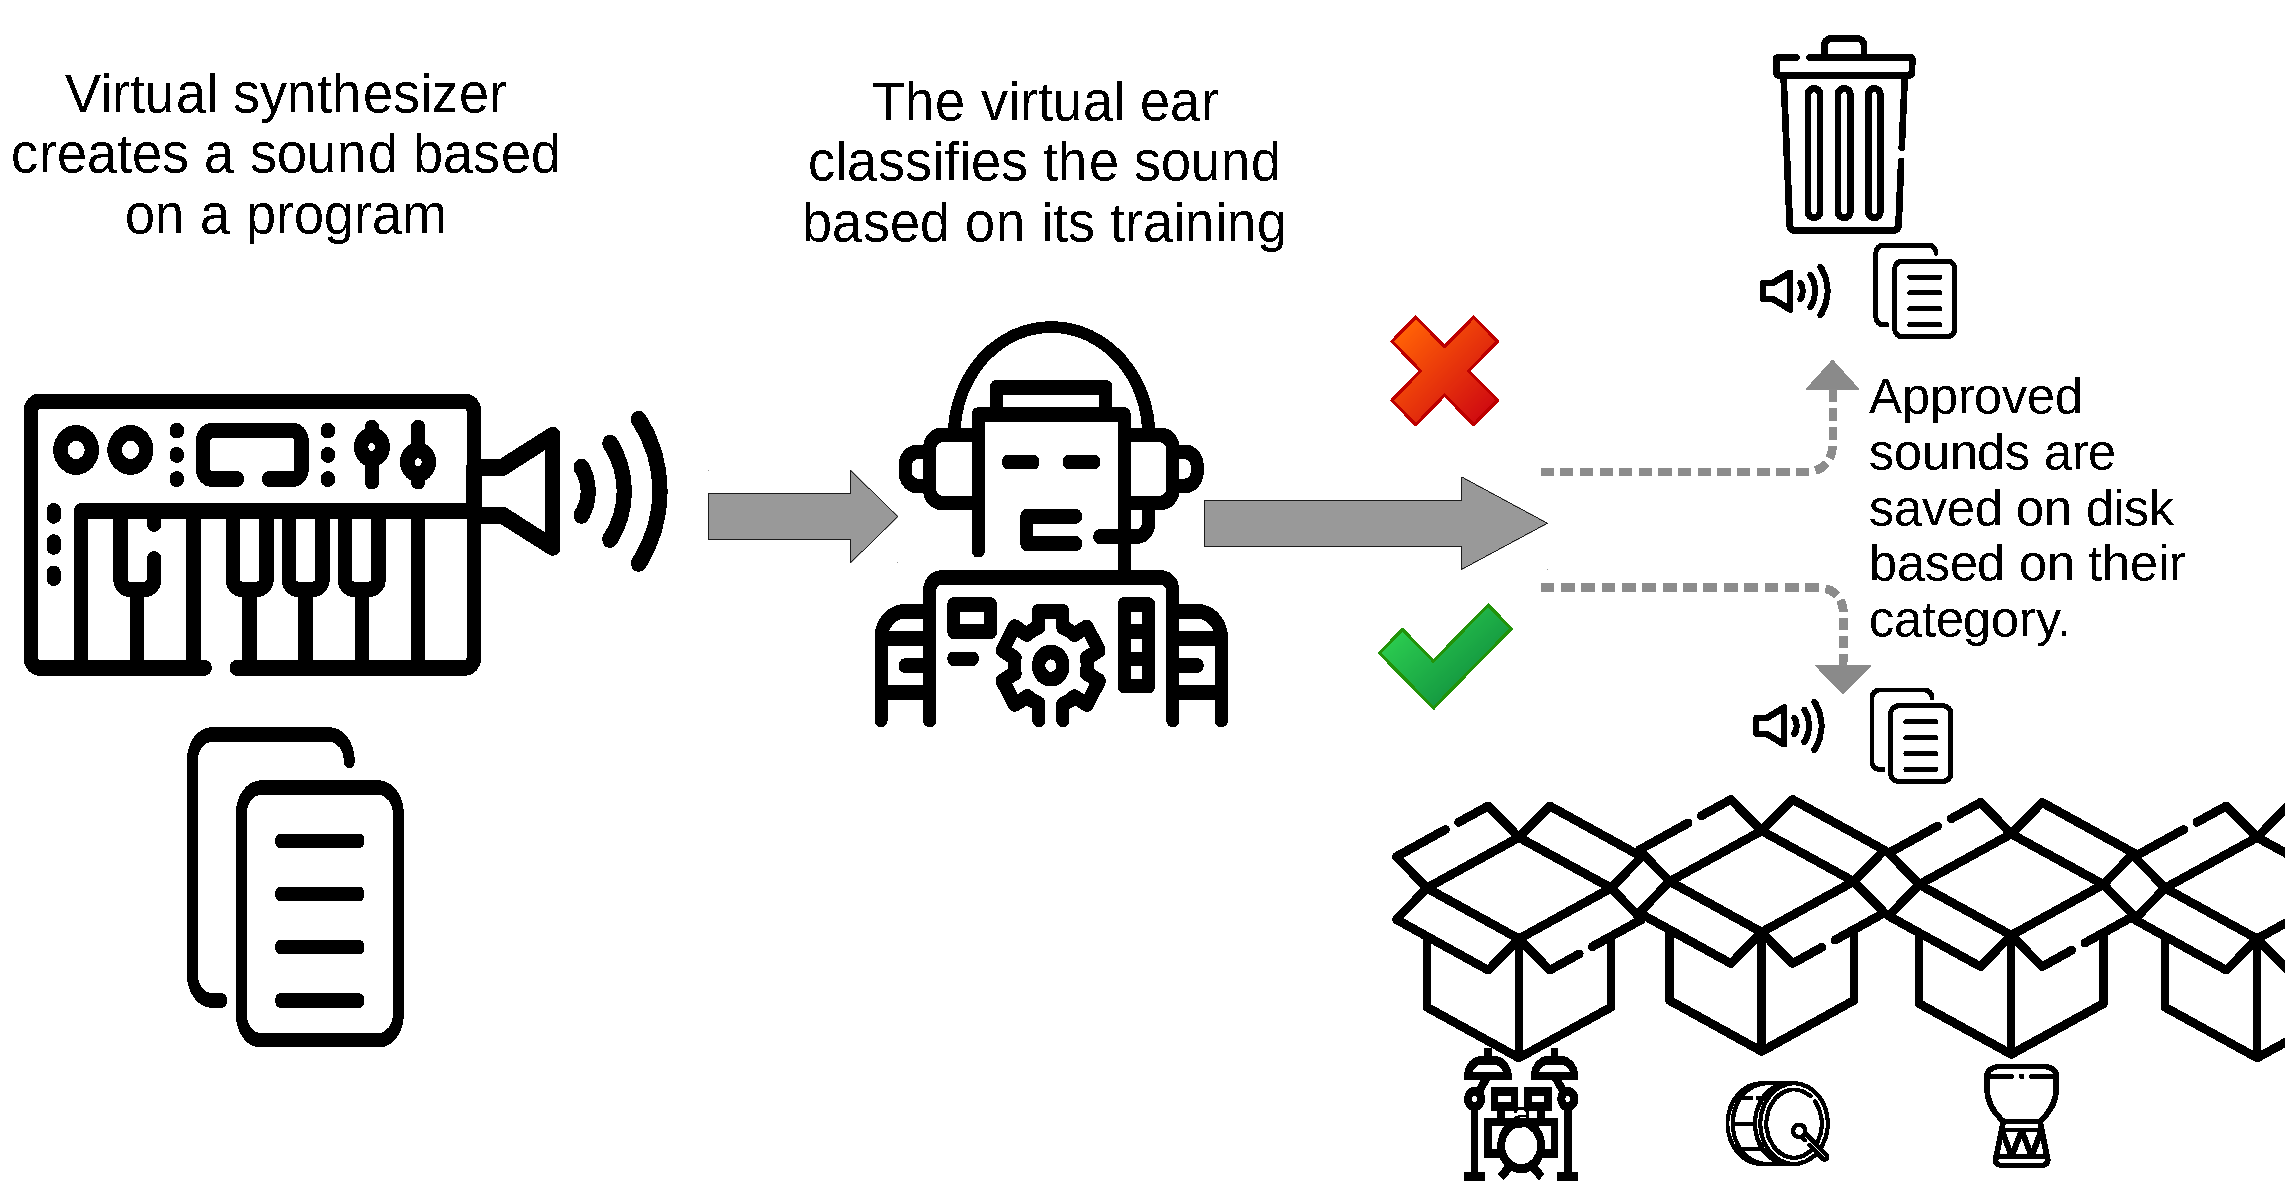
\includegraphics[width=1.1\linewidth]{images/chapter_4/pipeline.pdf}}}
    \end{center}
    \caption{A blueprint of our desired pipeline which allows each component to be implemented in a number of ways. Our implementation of this workflow also allows for easy parallelization when needed.
    }
\label{fig:pipeline_outline}
\end{figure}


\section{Virtual Synthesizer}
\label{vs}
 To create sounds, we need digital synthesizers capable of rapidly receiving or creating programs and rendering the corresponding sound offline. We use classical DSP to build our synthesizer, which allows for quick, offline, and parallel generation of audio signals without the usage of GPUs. We made extensive use of Pippi\footnote{https://github.com/luvsound/pippi} and SciPy~\cite{jones2001scipy} libraries. Our virtual synthesizer contains a set of one or more submodules. Each submodule is a self-contained noise making unit and creates signals by taking the steps depicted in figure~\ref{fig:submodule}. Submodules have identical sets of parameters, but widely different outputs can be achieved depending on the values assigned. The set of required parameters for each submodule is highlighted in Table~\ref{table:submodule_params}. The sonic output of the virtual synthesizer is the normalized addition of the output of its submodules. Our implementation of a synthesizer can have any number of submodules. We call the number of submodules in each virtual synthesizer the \textit{stack size}. We call the sets of parameter values that characterize a synthesizer's submodules a \textit{program} (analogous to presets and submodules for a VST).  

 \begin{figure}[htbp]
    \begin{center}
    % \textbf{Synthesizer SubModule }
    \makebox[\textwidth]{
    \fbox{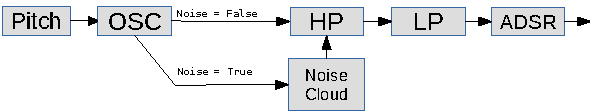
\includegraphics[width=1\linewidth]{images/chapter_3/synthesizer_block.pdf}}}
    \end{center}
    \caption{High level representation of pre-rendering steps for each submodule. Each Synthesizer contains 1 or more submodules. Synthesizer programs set the number of these submodules and their parameters.
    }
\label{fig:submodule}
\end{figure}

 \begin{figure}[htbp]
    \begin{center}
    % \textbf{Synthesizer SubModule }
    \makebox[\textwidth]{
    \fbox{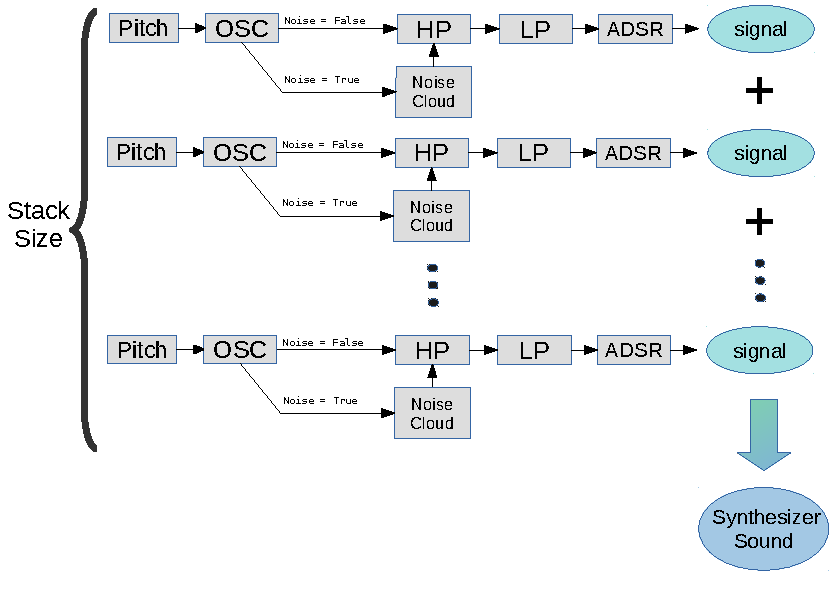
\includegraphics[width=1\linewidth]{images/chapter_3/synthesizer_all_blocks.pdf}}}
    \end{center}
    \caption{The output of the virtual synthesizer is the normalized addition of the output of its submodules. A synthesizer can have any number of submodules. 
    }
\label{fig:synth_modules}
\end{figure}
Our virtual synthesizer contains a set of one or more submodules. Each submodule is a self-contained noise making unit. Submodules have identical sets of parameters, but widely different outputs can be achieved depending on the values assigned. The set of parameters available to each submodule is highlighted in Table~\ref{table:submodule_params}. The sonic output of the virtual synthesizer is the normalized addition of the sonic output of its submodules. Our implementation of a synthesizer can have any number of submodules. The parameters that dictate the output signal of each submodule as well as the range of values each parameter can take are shown in table~\ref{table:submodule_params}. We call the number of submodules in each virtual synthesizer the \textit{stack size}. We call the sets of parameter values that characterize a synthesizer's submodules a \textit{program} (analogous to a preset for a VST).  

As we are interested in short, one-shot percussive sounds, each virtual synthesizer program will generate a 1 second piece of audio. This 1 second limit is over twice the length of the average one-shot drum sample within our database. Each submodule can make an audio signal with the length of 0.1-1 second, and play it at any point within the 1 second rendering time (but the entire sound must fit within the second, that is, a 0.5 second sound cannot begin playing after 0.5 seconds within rendering time frame). If the synthesizer has a stack size of more than 1 the audio signals from each submodule are overlapped and the total amplitude is normalized.

\begin{table}[t!]
\centering
\resizebox{\columnwidth}{!}{\begin{tabular}{ |c|c|c| } 
\hline
Parameters & Value Range & notes and constraints\\
\hline \hline
Attack & 0-3 & A-D-S-R values relative\\
Decay & 0-3 & relative to A-S-R\\
Sustain & 0-3 & relative to A-D-R\\
Release & 0-3 & relative to A-D-S\\
OSC type & sine,square,saw & tone type\\
IsNoise & boolean & whether to \newline use OSC type to generate noise\\
Length & 0-1 second & - \\
StartTime & 0-1 second & Length+Start$<$1\\
Amplitude & 0.1-1 & 1 = max amplitude\\
Pitches(notes) & list of pitches &  range of C0(16.35hz) to B9 \\
HP filter Cutoff & 0-20000hz & -\\
LP filter Cutoff & 20000-HP & never lower than HP cutoff\\
Filter Order & 4,8,16 & butterworth filter order \\
\hline
\end{tabular}}
\caption{Synthesizer submodule Parameters. Despite the simplicity of the parameters and our efforts at constraining the ranges, the number of parameters that can be randomly chosen for each submodule is in the order of $10^{15}$ }
\label{table:submodule_params}
\end{table}
The ADSR parameters shape the entire amplitude of the signal. Each submodule creates its signal at full amplitude then shapes it according to its internal ADSR parameter. Prior to being applied to the signal, each of these parameters is assigned an integer value in the range of 0-3, and normalized relative to the others such that \[ A_{norm} + D_{norm} + S_{norm} + R_{norm} = 1 \] \\ 
Where each value $v_{norm}$ in the $\{A_{norm}, D_{norm},S_{norm},R_{norm}\} $ set is normalized such that:
\begin{align*}
\text{for each $v$ $\epsilon$ \{A,D,S,R\}} \\
v_{norm} = \dfrac{v}{A + D + S + R}
\end{align*}
 The OSC type will determine the wave-shape of the signal. We limited this parameter to three fundamental wave forms: sine waves, square waves and saw waves. We also allow the creation of noise signals, which can imitate timbral characteristics of higher pitched drum samples at a very low computation cost (relative to the addition of thousands of sine waves at various frequencies). If the IsNoise boolean is set to true, the OSC type parameter loses importance as the OSC type will simply be used for the generation of noise via random wave-table transformations. Before the filter and ADSR envelope take affect, the generated noise will have similar characteristics to white noise. 

Each submodule is a monophonic synthesizer. That is, each submodule can play one note (or frequency) at a time. However, quick changes in pitch can occur in drum sound. Our more successful attempts at creation of synthetic kick or bass drums are often characterized by quick, exponential decrease of a sine-wave's pitch from medium to low audible frequencies. To mimic such sounds, synthesizer submodules may slide between 4 different pitches in the 1 second time frame. Each pitch value is a midi note with a frequency and length value. Each submodule accepts a list of 5 consecutive possible pitch values. The submodule will play each note in the list consecutively after normalizing the length values. The pitch notes are played in a portmanteau fashion such that there is no audible gap. This normalization of length values is similar to that of the ADSR values. 


\subsection{Is the Virtual Synthesizer Deterministic?}
\label{chap3:synth_deterministic}
It is crucial that the same set of synthesizer parameters result in identical, or near identical sounds. Our synthesizer modules are capable of producing random waves, or \enquote{noise}. This type of sound will vary each time it is produced. Manual listening does not show sonic variation between multiple creation of the same set of parameters, but how does this affect our ear models?

We create 50 parameter sets for stack sizes of 1 and evaluate each parameter set 10 times using the LSTM-DVN model. This model measures the probability of a sound belong to the drum/percussion category, and will be discussed in more detail in Section~\ref{TPE_models}. Put simply, we are creating the sonic output of the same parameter set multiple times and measuring its effect on one of our models. We repeat this experiment for stack sizes of 2 and 8 and show the results in figure~\ref{fig:synth_deterministic}.

\begin{figure}[htbp!]
\begin{center}
    \textbf{ Variation in Repeated Evaluations of Parameters }\par\medskip
    \makebox[\textwidth]{
    \subfloat[1 Stack]{ 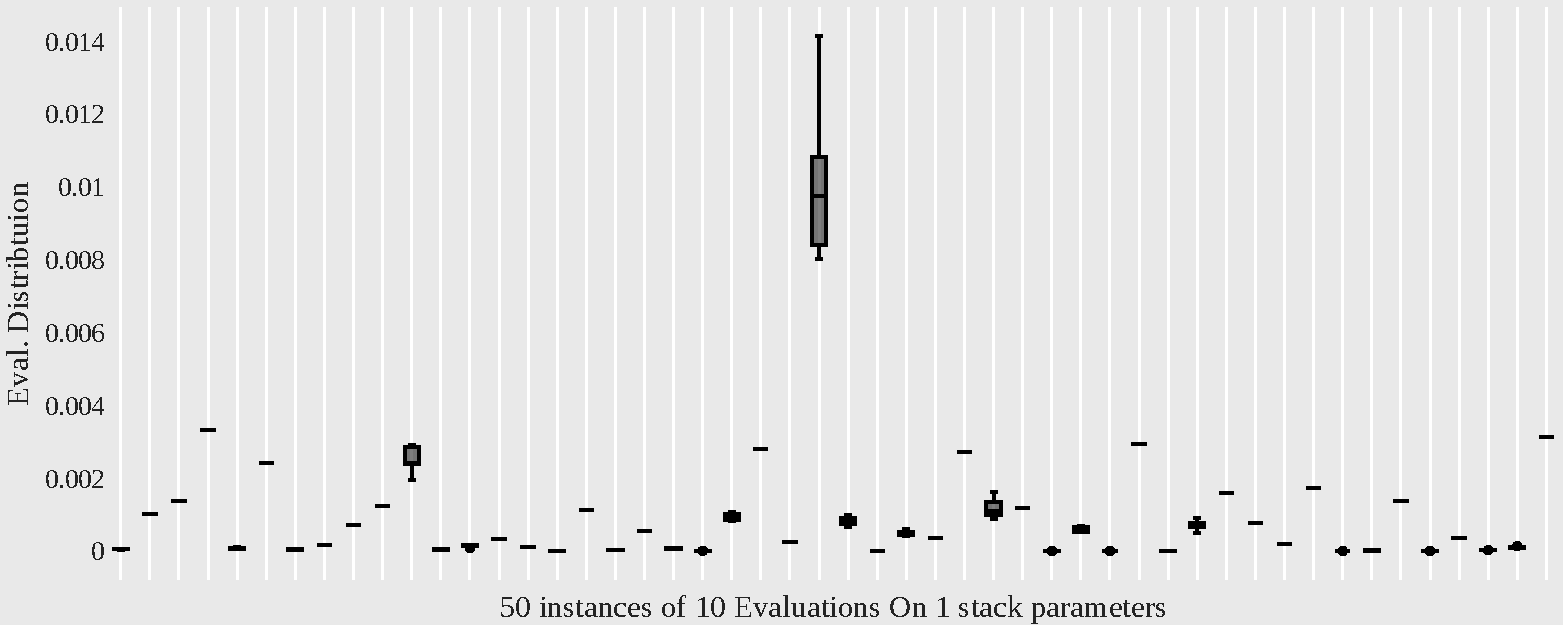
\includegraphics[width=17cm,height=5.67cm]{images/chapter_3/eval_stability_stacksize1.pdf}

    }}

    \makebox[\textwidth]{
    \subfloat[2 Stacks]{ 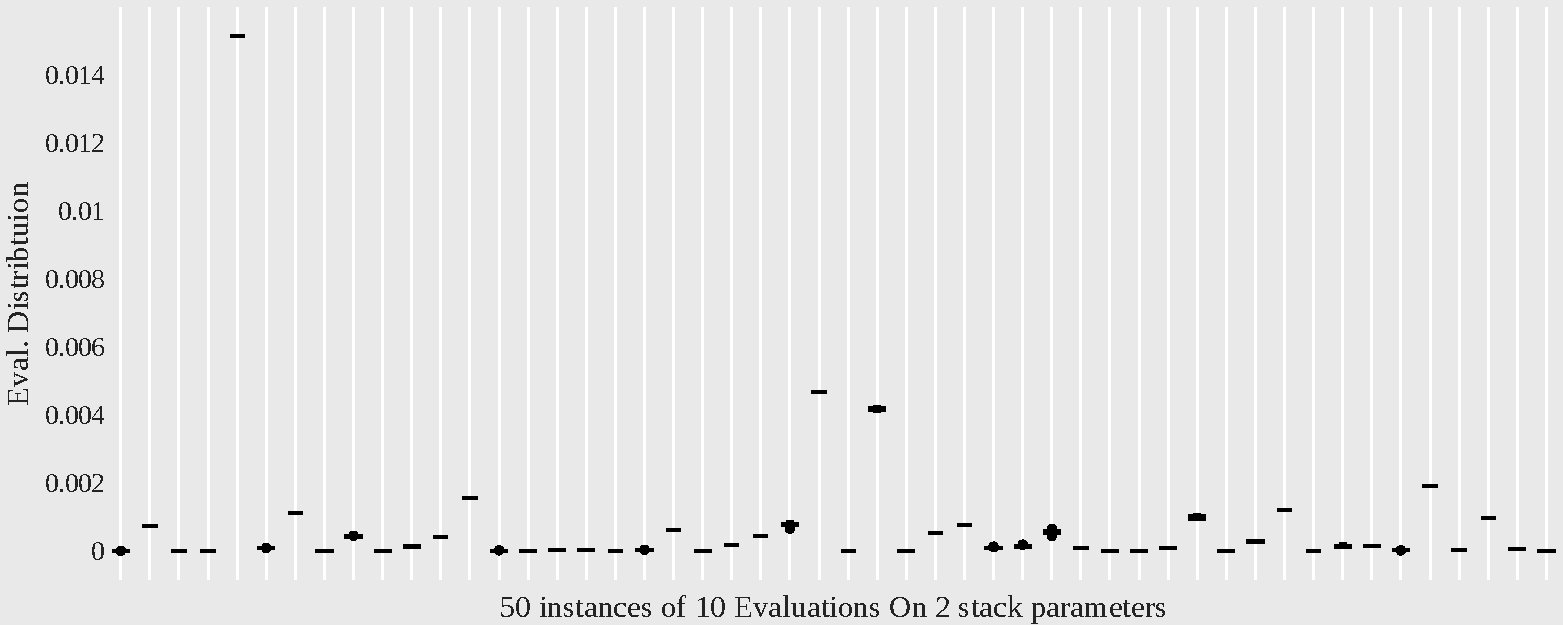
\includegraphics[width=17cm,height=5.67cm]{images/chapter_3/eval_stability_stacksize2.pdf}

    }}
    
    \makebox[\textwidth]{
    \subfloat[8 Stacks]{ 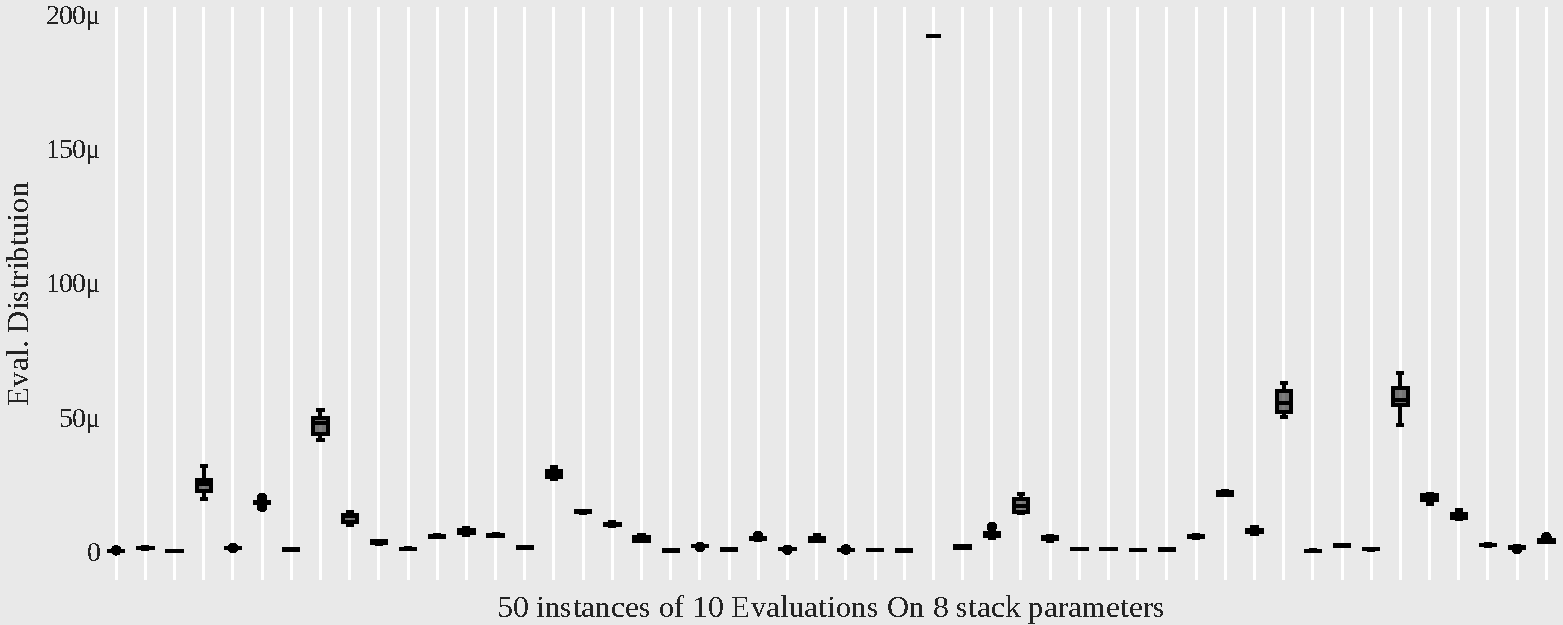
\includegraphics[width=17cm,height=5.67cm]{images/chapter_3/eval_stability_stacksize8.pdf}

    }}
\end{center}

\caption{Repeated evaluation of signals from identical paramter-sets shows little variation in scores. Multiple renditions of the same parameter-set vary if the parameter-set calls for generation of 1 or more random wave-shapes. We do not believe these variations to be significant.}
\label{fig:synth_deterministic}
\end{figure}


\section{The Ear}
What we refer to as an \enquote{ear} is any method of scoring and classifying audio (e.g machine listening) \cite{malkin2006machine,rowe1992interactive}. The ideal ear for our task will be capable of receiving a piece of audio and giving it a score (or a list of scores) based on how well it satisfies certain criteria. In this work we are mainly focused on generation of novel percussive sounds, therefore, what we require from the ear is to give us probabilities of an audio sample belonging to various categories. Our synthesizer outputs are close to deterministic for all programs, therefore evaluations of the ear would allow us to associate scores of the sound with the parameter values (or program) that generated it. In Section~\ref{gens} we discuss how these scores can be used to navigate synthesis towards parameters which give us the desired sonic output.

We are not looking for the perfect imitation of organic drums using a synthesizer. We seek to imitate drums using a synthesizer and even \textbf{prefer} for its generations to retain novel, unusual characteristics. The task assigned to the virtual ear is the rare acceptance of drum-like sounds and the inevitable rejection of most \enquote{noise} outputs from the virtual synthesizer. By definition, we cannot anticipate what these novel drums will sound like. All we know is that the accepted sounds are synthesizer noises which the synthetic ear has determined to be similar to drum-sounds. 

Figure~\ref{fig:ven_data} highlights a critical problems with this approach. we denote $\mathcal{N}$ as the set of percussive sounds a synthesizer is capable of making. $\mathcal{T^{+}}$, our positive examples of what percussive instruments sound like is a set of sound extracted from material drums. $\mathcal{T^{-}}$, is a small subset of an infinite set which is meant to represent all noises which the synthesizer is capable of making. It likely includes a number of sounds which to our ears could be used as drums. During the hearing test, the virtual ear continually receives synthesizer noises ($\mathcal{H}$) for classification. The performance of the ear is measured by its precision and recall in finding the overlap between $\mathcal{H}$ and $\mathcal{N}$. It is critical to ensure that the change in learning domains---particularly with the case of positive examples of percussive instruments---does not interfere with transformation of knowledge from the training of the ear to the hearing test. To maximize the transference of knowledge from one domain to another, we seek to learn from agnostic feature sets that capture fundamental characteristics of the data points. 

 With our dataset of labeled drum sounds, discussed in Section~\ref{sec:data}, we implement several well performing algorithms for categorizing unlabeled drum sounds, given that we know they are drum sounds. However, a major hurdle towards the implementation of a \textquotedblleft drum from non-drum \textquotedblright recognizing ear is that the set of sounds that are not percussive is infinite. In this project we treat the variety of sounds created by the virtual synthesizer as an infinite set and seek to represent the \enquote{not drum} set with as few samples as possible.

 
In our case, drum groups are an example of closed sets, since we believe that a sufficiently large sample pack can effectively describe common drum categories. However, effective representation of all possible non-drum sounds is not attainable via examples alone. We hypothesize that a major subtask in the implementation of our virtual ear falls outside the traditional categorization problem and within the \enquote{Open Set Recognition} (OSR) domain~\cite{geng2020recent,mundt2019open}. 

Traditional classification tasks often make the assumption the data points used for training the model and future unlabeled data will emerge from the same system of processes~\cite{geng2020recent,mundt2019open}. This assumptions requires that sufficient positive examples of all possible classes exist and are trained on. Works toward the implementations of GANs have documented scenarios in which networks will assign high categorization probabilities to nonsensical, out of context data which should be rejected rather than categorized~\cite{geng2020recent,mundt2019open,hassen2020learning}.  
 Once a sound is generated and passed onto the ear, we expect the virtual ear to facilitate our actions in response to two important questions: 
\emph{
\begin{quote}
\text{Decision.1 Could the sound be used as a drum?}\label{Decision.1}
\\
\text{Decision.2 If it does sound like a drum, what type of drum should it be?}\label{Decision.2}
\end{quote}
    }


\hypref{Decision.1} requires knowledge of what drums \textbf{do not} sound like, or knowledge of an infinitely large set, which cannot be fully represented via examples. An important consideration is that the source of sounds used in training the model (organic drum sounds) will be fundamentally different from the source of unlabeled sounds we wish to categorize (noise from a synthesizer). Much easier to answer is \hypref{Decision.2}, where we found satisfying results with a variety of different approaches. We attribute the relative ease of \hypref{Decision.2} relative to~\hypref{Decision.1} to be reflective of the OSR problem. 

Our goal is to create a pipeline of sound generation where the synthesizer is used for the rapid generation of sounds and the virtual ear is used for the acceptance of inputs which satisfy some fundamental characteristics of percussive instruments. How we characterize this description is critical as it allows novel sounds to be accepted as part of the drum group despite their anomalies. We approached this problem by the implementation of various feature extraction methods as well as various models which use these features towards a solution for ~\hypref{Decision.2} and~\hypref{Decision.1}.

We cover the implementation of these virtual ear models in two sections: \emph{two phased ears} (TPEs) and \emph{mixed ear models} (MEMs). TPEs are a combination different models for each of ~\hypref{Decision.2} and~\hypref{Decision.1}. The features utilized by these models are manually defined. mixed ear models use a highly compressed, automatically encoded representation of sound to give simultaneous answers to both questions.

\begin{figure}[htbp!]
    \begin{center}
    \textbf{Data Overview}
    \makebox[\textwidth]{
    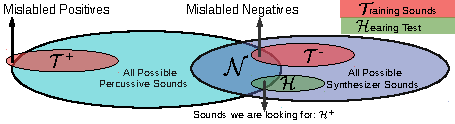
\includegraphics[width=1\linewidth]{images/chapter_4/venn_data.pdf}}
    \end{center}
    \caption{ An illustration of the discrepancy between the sounds we use to train our classifiers and the type of sounds the classifier is expected to classify. $\mathcal{N}$ is the set of percussive sounds a synthesizer is capable of making. The inclusion of sounds in this group may vary from person to person. Our positive samples, $\mathcal{T^{+}}$, is a small fraction of a wide variety of percussive sounds that are conceivable. For $\mathcal{T^{-}}$, we can generate any number of random samples. $\mathcal{H}$ is a series of sounds sent to the ear for classification.}
\label{fig:ven_data}
\end{figure}
\subsection{Two Phased Ears}
\begin{figure}[t!]
    \begin{center}
    \textbf{TPE Design}
    \makebox[\textwidth]{
    \fbox{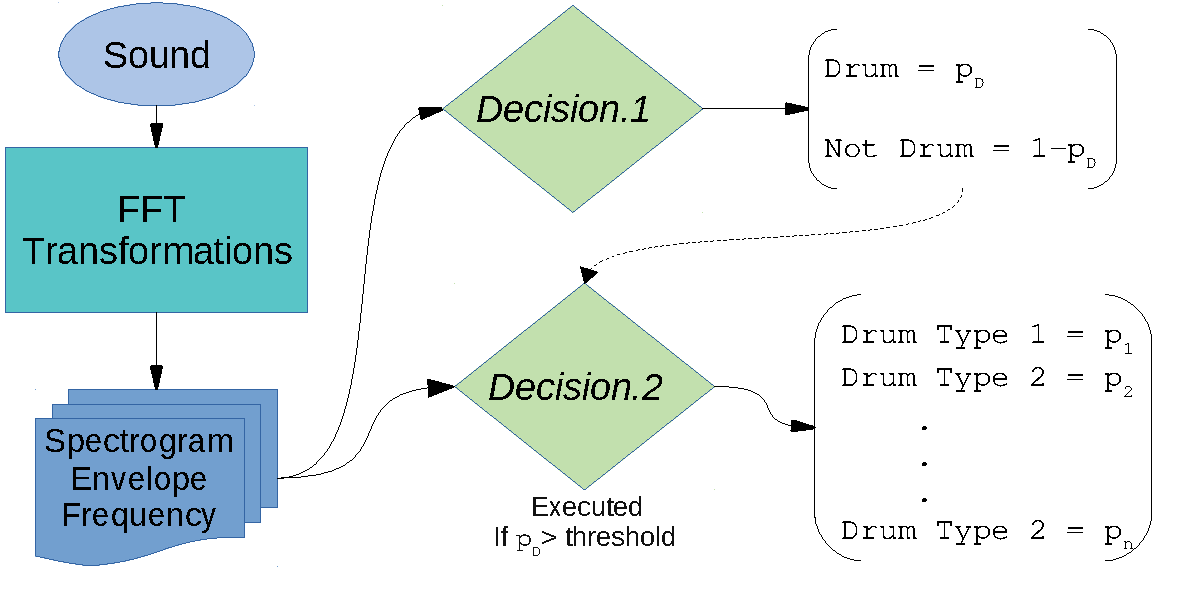
\includegraphics[width=1.1\linewidth]{images/chapter_4/TPE_ear.pdf}}}
    \end{center}
    \caption{TPE's receive a sound and make decisions sequentially.}
\label{fig:TPE_design}
\end{figure}

\label{sec:ear}

%\lstset{language=Python}
\label{TPE_models}
% Default fixed font does not support bold face

\lstset{escapeinside={@(}{)@}}

Using the described features, we trained several neural network models for Phase 1 and 2 in the Pytorch environment. The task of Phase 1 is to separate drums from not-drums (DrumVsNotDrum, or DVN). The task of Phase 2 is to categorize drums and percussion (DrumVsDrum, or DVD). We kept our feature space small, making it viable for feature selection and model design to be done on a trial and error basis. For all models, accuracy is calculated by prediction of all test dataset labels and the loss function and optimizer are Categorical-CrossEntropy and Adam respectively. Training continues until no reduction in loss and accuracy is observed in 10 epochs. 


\subsubsection{DVN Models}
\textbf{FC-DVN}: Fully connected network trained on Envelope features, reaching 97\% accuracy on our test data for Phase 1. With size of 10x5x10. \\
\begin{center}
\vbox{
    \begin{lstlisting}[caption=Sequential Layers for CNNLSTM-dvn]
            Layer                       Details
            ========================================================
            Linear                      in_features=400 
                                        out_features=20 
                                        bias=True
            PReLU                       
            Linear                      in_features=20
                                        out_features=10 
                                        bias=True
            PReLU
            Linear                      in_features=10
                                        out_features=4
                                        bias=True
            PReLU
            Linear                      in_features=4
                                        out_features=2
                                        bias=True
            Softmax                     DVN probabilities
                        
        \end{lstlisting}}
\end{center}
\textbf{CNNLSTM-DVN}: A combination of CNN and LSTM models, where the CNN model extracts higher level features that are fed temporally to an LSTM cell. This model is trained on spectrum data and reaches 98\% accuracy on our test set. Its structure is the combination of a CNN with 2 output channels and kernel size $(7,3)$; Followed by an LSTM model of hidden size 800 and a fully connected layer of size 20x2.\\
\begin{center}
\vbox{
    \begin{lstlisting}[caption=Sequential Layers for CNNLSTM-dvn]
            Layer                       Details
            ========================================================
            Conv2d                  kernel size = (7, 3)
                                    stride = (1, 1)
                                    padding = (3, 1)
            ReLU
            Dropout                 probability = 0.5
            LSTMCell                hidden size = 800
                                    input size = @($\mathcal{F}$)@
            Linear                  in_features = @($\mathcal{F}$)@
                                    out_features = 2
                                    bias=True
            Softmax                 DVN probabilities
\end{lstlisting}}
\end{center}

\subsubsection{DVD Models}
\textbf{E+F-DVD}: A fully connected model trained on a concatenation of envelope and frequency features. Reaching 80\% accuracy for 6-way drum categorization in Phase 2. Size of 50x10x2x6.\\
\begin{center}
\vbox{
    \begin{lstlisting}[caption=Sequential Layers for CNNLSTM-dvn]
            Layer                       Details
            ========================================================
            Linear                      in_features = 10+50 
                                        out_features = 30
                                        bias = True
            PReLU                       
            Linear                      in_features = 30
                                        out_features = 10
                                        bias = True
            PReLU                       
            Linear                      in_features = 10
                                        out_features = 10
                                        bias = True
            PReLU     
            Linear                      in_features = 10
                                        out_features = @($\mathcal{C}$)@
                                        bias = True
            Softmax                     drum type probabilities
        \end{lstlisting}}
\end{center}

\textbf{CNN-DVD}: A CNN model trained on Spectrum features. Reaching 82\% accuracy in a 6-way drum categorization in Phase 2. A combination of a CNN model with output channel size of 4, kernel of size of 5, another CNN model with output channel size of 8 and kernel of size 3. Followed by a fully connected network of shape 100x20x6.\\ (WRONG ARCHITECTURE IN CODE)
\begin{center}
\vbox{
    \begin{lstlisting}[caption=Sequential Layers for CNNLSTM-dvn]
            Layer                       Details
            ========================================================
            Conv2d                  kernel size=(7, 3)
                                    stride=(1, 1)
                                    padding=(3, 1)
            ReLU
            Dropout                 probability=0.5
            LSTMCell                hidden size=800
                                    input size=20
            Linear                  in_features=20
                                    out_features=@($\mathcal{C}$)@
                                    bias=True
            Softmax                 drum type probabilities
        \end{lstlisting}}
\end{center}

\textbf{FC-DVD}: Fully connected 3 layer neural net with 78\% accuracy for 6-way drum categorization in Phase 2. Size of 400x200x50.
\begin{center}
\vbox{
    \begin{lstlisting}[caption=FC-DVD]
            Layer                       Details
            ========================================================
            Linear                      in_features=400
                                        out_features=20 
                                        bias=True
            PReLU                       
            Linear                      in_features=20
                                        out_features=10 
                                        bias=True
            PReLU
            Linear                      in_features=10
                                        out_features=4
                                        bias=True
            PReLU
            Linear                      in_features=4
                                        out_features=@($\mathcal{C}$)@
                                        bias=True
            Softmax                     drum type probabilities
                        
        \end{lstlisting}}
\end{center}
\subsubsection{Creating An Ear}
The parameters are hand-picked and un-tuned. As discussed in Section~\ref{surveys}, higher accuracy rates in these models do not translate to higher agreeableness with humans. leading us to believe that model accuracy on test data alone cannot be relied upon when the domain of sounds 
being categorized is switched from original percussion samples to virtual synth sounds.

With our models showing high accuracy on testing data, we combine models in order to increase the efficacy of each phase and address the \enquote{open set problem} for our task. For Phase 1 we only determine sounds as percussive if both FC-DVN and CNN-LSTM have determined it as such with over 90\% confidence. For the majority of our random generations that is not the case, but if a randomly generated sound has passed this phase, our three categorizers assign their categorizations to this sound. These categorizers have a moderate degree of agree-ability as seen in~\ref{surveys}, but often the decision is not unanimous. The fourth method of categorization, \enquote{averaged-cat}, is implemented by taking the sum of the softmax outputs of all three categorizers, using it to determine the category. 

These models can be combined and weighted in various ways and the confidence thresholds can be modified in order to implement \enquote{virtual ears} with different properties. A glaring issue in the current implementation is the treatment of softmax outputs as a reasonable measure of a model's confidence. As a result, some models may have unwarranted higher confidence in their scores, skewing attempts at finding a consensus. 
\subsection{Mixed Ear Models}

\begin{figure}[t!]
    \begin{center}
    \textbf{MEM Design}
    \makebox[\textwidth]{
    \fbox{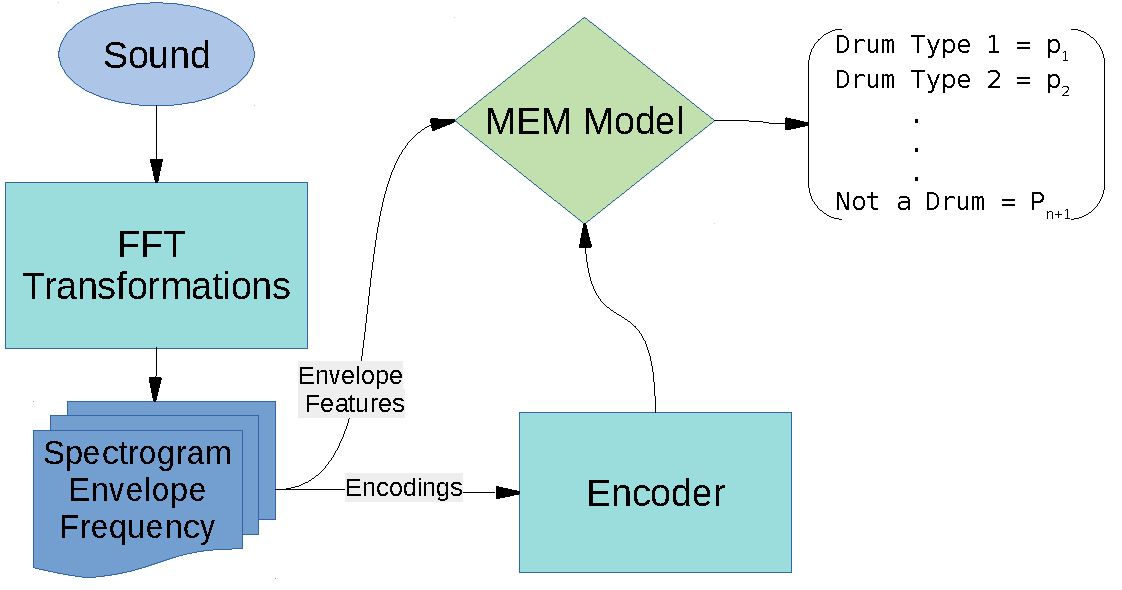
\includegraphics[width=1.1\linewidth]{images/chapter_4/MEM_ear.pdf}}}
    \end{center}
    \caption{MEMs use both FFT features and embedding features to make both decisions simultaneously. }
\label{fig:TPE_design}
\end{figure}
\label{chap3:mixed_ear_models}
As t-SNE results are not classifiers in of themselves, we create a model which uses encoded versions of each sound group to predict its type. This differs from two-phased ears as we are simultaneously categorizing a new sound's drum type or putting it in the \enquote{synthetic noise} category. We call this task drum vs drum vs not-drum, or \enquote{DvDvN}. We also tackle the Drum vs Not-Drum problem using our embedding features.

As discussed in Section \label{fig:embedding_FE}, manual t-SNE inspections highlighted the disregard for envelope shapes as a major source of failure. We compare the performance of our models before and after the addition of envelope features (a vector of size 10) to the feature space. 

We reuse the model trained on  MixedDB as our embedding feature extractor. We use a combination of RadarDB, FreeDB and NoiseDB for training. We only focus on clap,hat,kick,snares, synthetic noise groups for measuring effectiveness to prevent class overlaps as much as possible. We also exclude samples longer than 1 second, to exclude potentially mislabeled data. Our final training database for mixed ear models is described in table~\ref{db:memDB}.
\begin{table}[htbp]
\centering
\begin{tabular}{|l|l|l|l|l|l|}
\hline
 DB Name & kick & snare & clap & hat & Synthetic Noise\\\hline
 MixedEarDB & 1334 & 1035 & 401 & 1275 & 1000 \\ \hline
\end{tabular}
\caption{MixedEarDB: A database put together by combination of radarDB, FreeDB and NoiseDB}
\label{db:memDB}
\end{table}

\subsubsection{Model Selection}
Using our encoding and envelope features to represent audio, five classification models were trained for the task of categorizing the five different sound groups. For hyper-parameter optimization, the models were trained using 5-fold cross validation and 80/20 train-to-test ratio. The F-Score result of each cross-validation is the unweighted average F-Score of all groups. For inter-model comparisons, the procedure is the same except 10-fold cross validations are used. Our models were derived from scikit-learn's implementations of these classifiers~\cite{pedregosa2011scikit}. Before inter-model comparisons, we conducted a grid-search for each model on at least one of its possibly decisive hyper-parameters. The classifiers and other notable specifications are presented in table~\ref{table:mem_model_selection}. We introduced class weights where possible to mitigate the effects of an imbalanced dataset~\cite{provost2000machine,chawla2004special}. When utilized, the weight for each class $c$  is calculated as:

\begin{subequations}
    \begin{align*}
    c_{weight} = 1-\dfrac{\text{number of samples in group $c$} }{\text{Total number of samples}}
    \end{align*}
\end{subequations}

\begin{table}[t]
    \centering \hspace*{-0.8cm}
    \begin{threeparttable}
    \begin{tabular}[width=0.95\paperwidth]{|l|l|l|}
    \hline
    Model name & Tuned Parameters\tnote{\dag}  & Used Weights? \tnote{\ddag} \\\hline
     Support Vector Classifier (SVC) &  Gamma:0.001, C:100, kernel:rbf & Yes\\
     LinearSVC & C:10 & Yes\\
     K Nearest Neighbors & Num. Neighbors:31 &  No \\
     Random Forest Classifier & Num Estimators:500 & Yes \\
     Extra Trees Classifier & Num Estimators:1100 & Yes\\
     \hline
    \end{tabular}
    \caption{Models implemented for comparison using envelope and embedded features. }
    \begin{tablenotes}
    \item[\dag] Tuned parameters values are based on grid-searching for best f-score. Parameters not mentioned have neither been tuned nor changed from scikit-learn's default values (as of version 0.23)
    \item[\ddag] Class weights are used unless not applicable to classifier.
    \end{tablenotes}
    \label{table:mem_model_selection}
    \end{threeparttable}
\end{table}

\begin{figure}[htbp!]
    \begin{center}
    \textbf{Cross Validation F-Scores For All Sound Groups}\par\medskip
    \makebox[\textwidth]{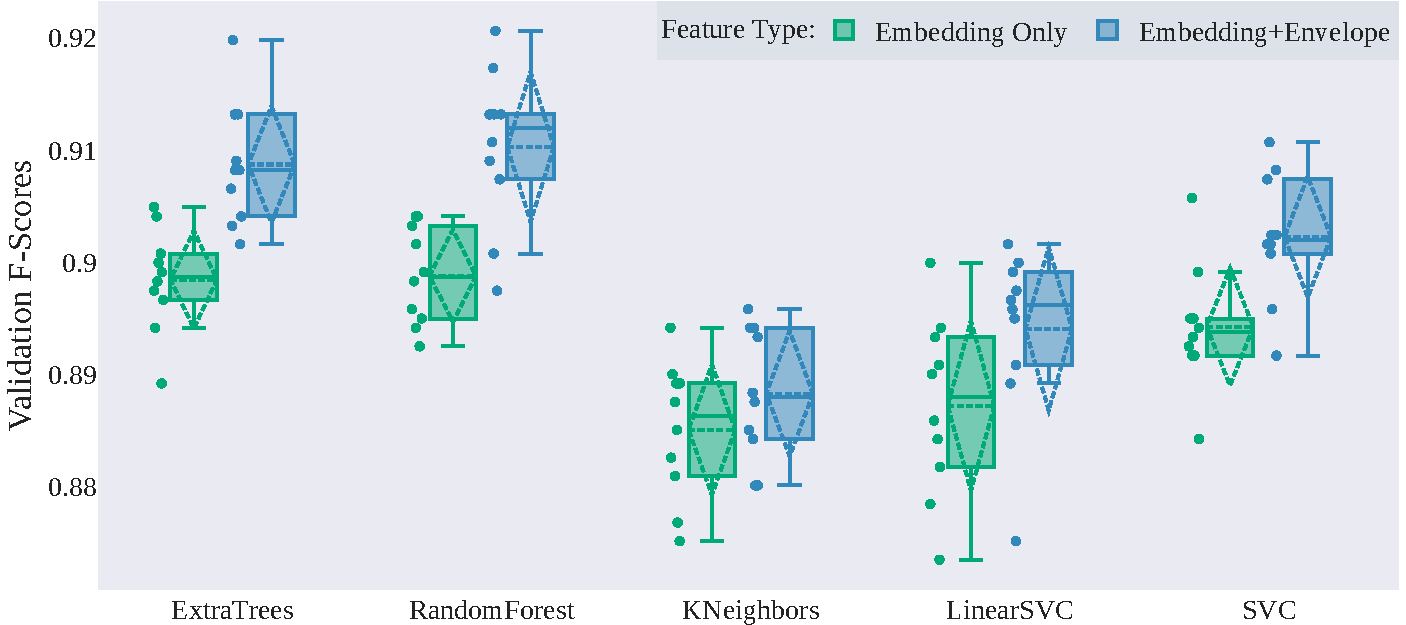
\includegraphics[width=0.8\paperwidth]{images/chapter_3/mme_comparisons_mme.pdf}}
    \caption{Boxplots visualizing the F-Score results for each cross-validation. The individual scores, means, medians, standard-deviation and outliers are depicted. The differences are noticeable, yet means lie within the \%88-92 range. Envelope features improve classification accuracy for all models. }
    \label{fig:f1_allg_box}
    \end{center}
\end{figure}

We're also interested in how these models perform on the binary drum vs not drum task.
After grouping all drums together, we repeat the model selection process above. We also repeat the hyper-parameter optimization step where no changes appeared necessary except for a reduction in the number of neighbors for the K-Neighbor model (from 30 to 5). As show in in figures~\ref{fig:f1_allg_box} and~\ref{fig:f1_dvn_box}, the addition of envelope features had a positive effect on performance for all mdoels, yet the RandomForest and ExtraTrees models clearly outperform the other classifiers in both tasks. We train the top two models on \%80 of our database and use the remaining \%20 to create the confusion matrices and the F-Scores shown in figures~\ref{fig:conf_f1_dvn}.
\begin{figure}[h!]   
    \begin{center}
        \textbf{Cross Validation F-Scores For Drum Vs Not-Drum}
    \makebox[\textwidth]{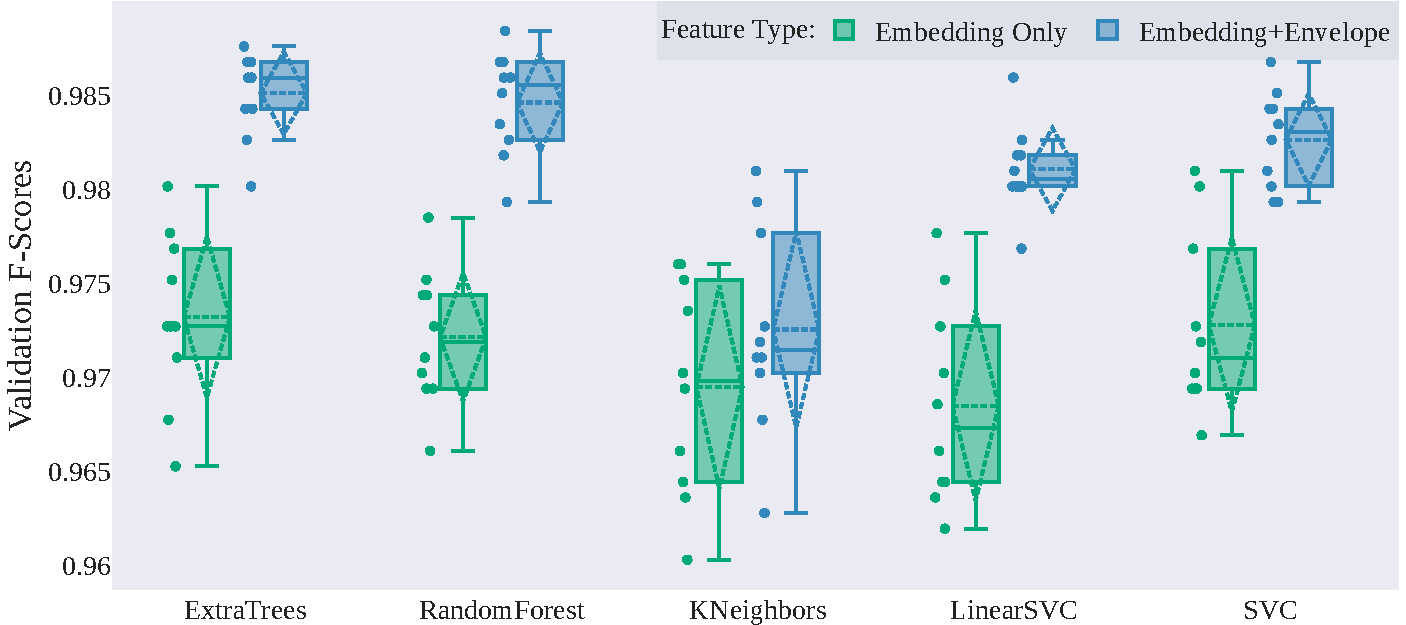
\includegraphics[width=0.8\paperwidth]{images/chapter_3/mme_comparisons_dvn.pdf}}
    \caption{F-Score results for each cross-validation. Models perform better as there are less categorization groups. Envelope features increase accuracy for all models. Random Forest and Extra Trees remain the top two models. }
    \label{fig:f1_dvn_box}
    \end{center}
\end{figure}


\begin{figure}[htbp!]
\begin{center}
    \textbf{ Classification Report for DvDvN and DvN  }\par\medskip
    \makebox[\textwidth]{
    \subfloat[Precision, recall, F1-Score, and number of supporting examples]{ 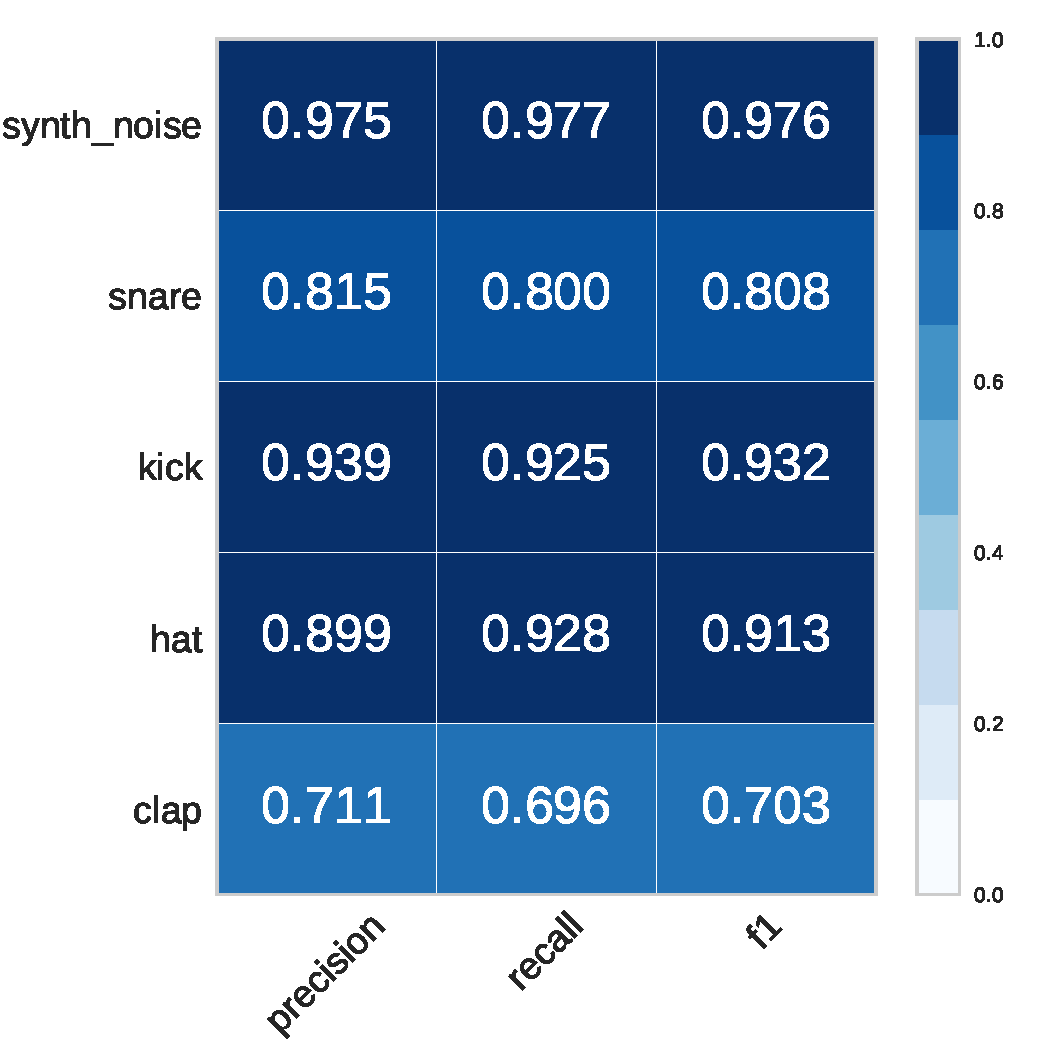
\includegraphics[width=9cm,height=9cm]{images/chapter_3/f1_mme.pdf}
    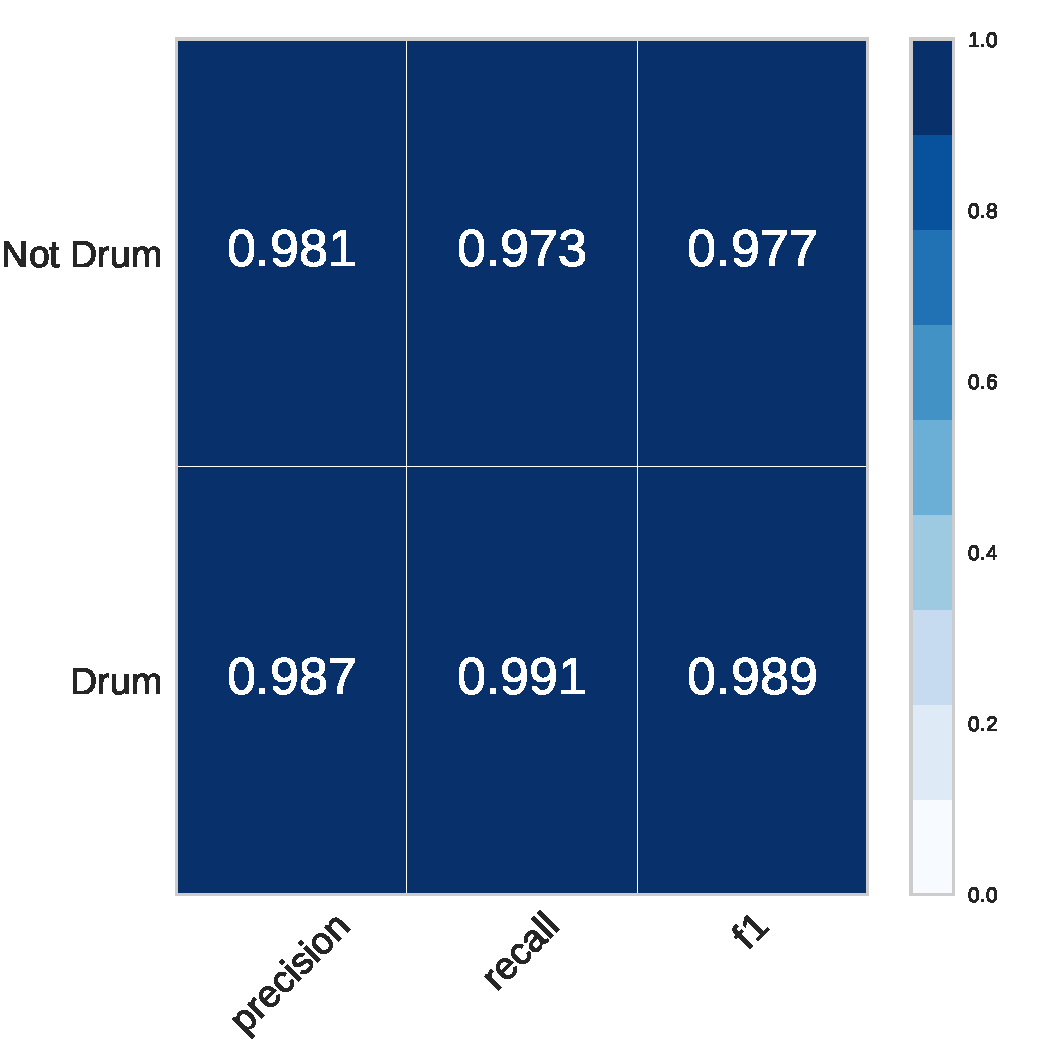
\includegraphics[width=9cm,height=9cm]{images/chapter_3/f1_dvn.pdf}
    }
    
    }
\label{fig:conf_f1_dvd}
\end{center}

\begin{center}
    \makebox[\textwidth]{
    \subfloat[Confusion matrices]{ 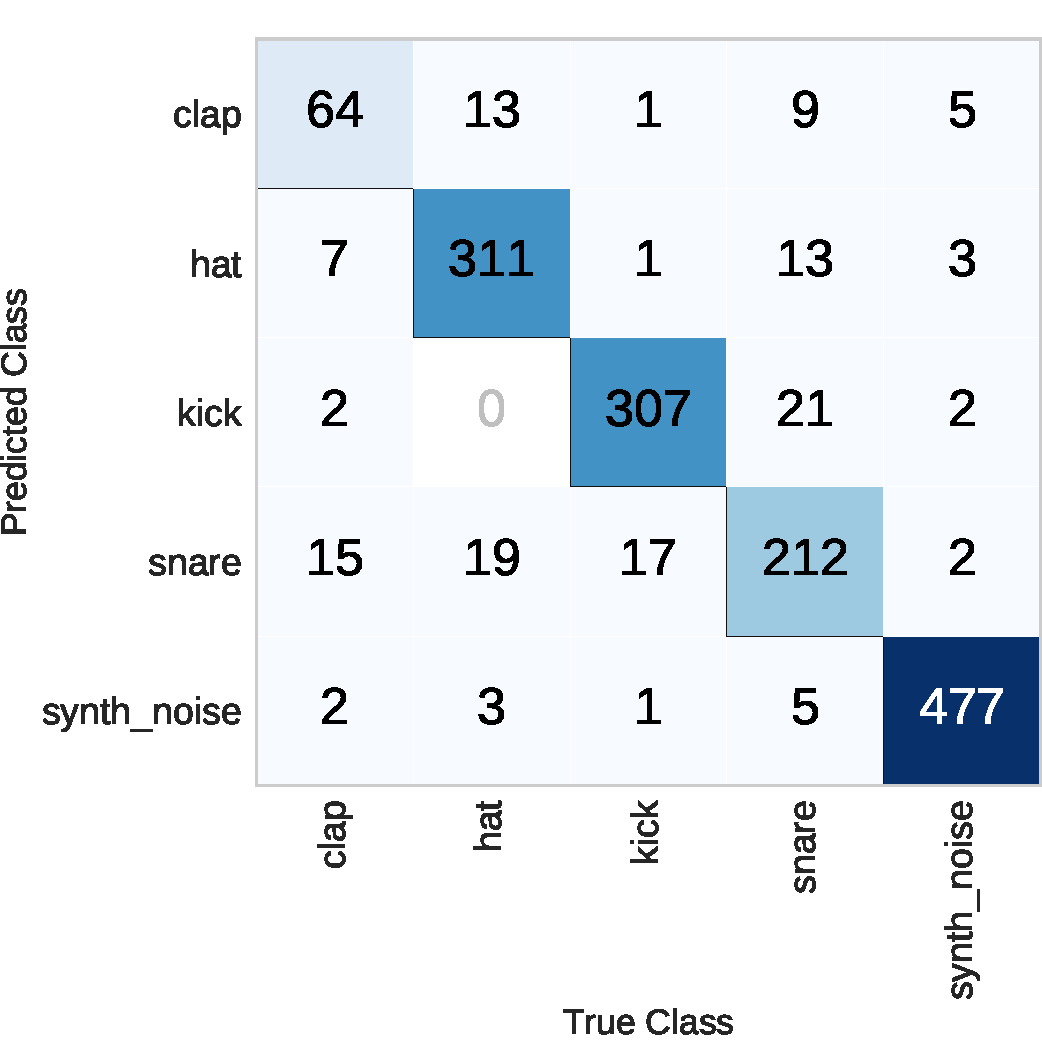
\includegraphics[width=9cm,height=9cm]{images/chapter_3/conf_mme.pdf}
    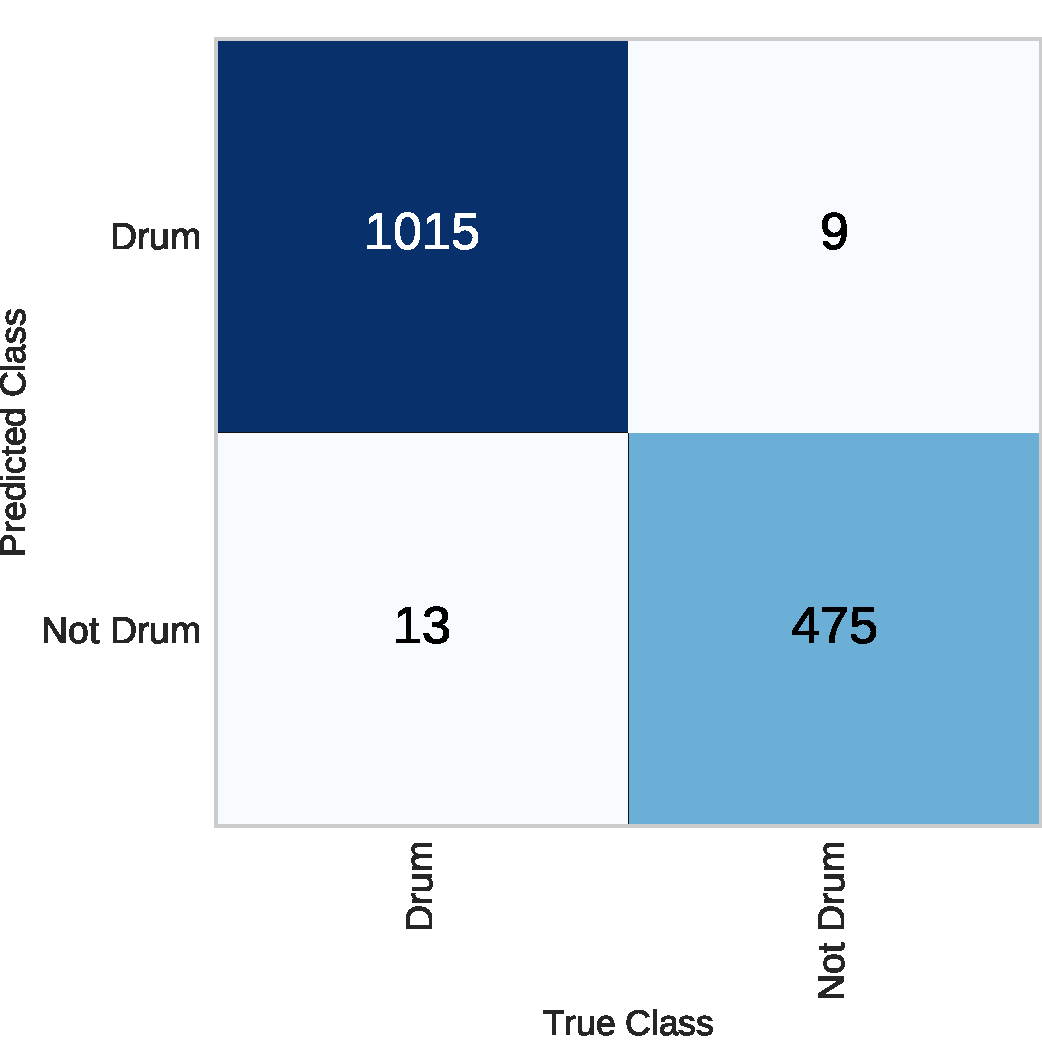
\includegraphics[width=9cm,height=9cm]{images/chapter_3/conf_dvn.pdf}
    }}
\end{center}


\caption{F-Scores and confusion matrix of ExtraTrees model for both DvDvN and drum vs not-drum categorization.}
\label{fig:conf_f1_dvn}
\end{figure}

Based on these reports, having multiple options for drum categorization does not noticeably influence our models accuracy in categorizing synthetic noise as synthetic noise. However, the DvDvN models's slightly smaller false negative rate for synthetic noise (11 vs 13 false negatives) is countered by a slightly higher rate of categorizing drums as synthetic noise (12 vs 9).  We therefore use the DvDvN implementation as it simultaneously categorizes drum types and separates noise from drums. However, without manual inspection, we cannot confirm the extent of this model's usefulness. 

We create the mixed ear model by combining our encoder with the ExtraTrees classifier. As sounds are generated with the virtual synthesizer, the encoding and envelope features will be extracted using the encoder and sent to the ExtraTrees DvDvN classifier. In the upcoming novel generations Section, we will present the results of a two person survey where the accuracy of the two-ear model is analyzed given 500 synthetic noise sounds categorized as drums. 





\end{document}